\chapter{Introduction}
\label{chap:introduction}

% This is the introduction where you should introduce your work. In
% general the thing to aim for here is to describe a little bit of the
% context for your work -- why did you do it (motivation), what was the
% hoped-for outcome (aims) -- as well as trying to give a brief overview
% of what you actually did.
%
% It's often useful to bring forward some ``highlights'' into this
% chapter (e.g.\ some particularly compelling results, or a particularly
% interesting finding).
%
% It's also traditional to give an outline of the rest of the document,
% although without care this can appear formulaic and tedious. Your
% call.



% \section{Context}
% \label{sec:context}
% % "describe a little bit of the context for your work"


% Hook (Compilers and compiler frameworks)
Compilers are a critical component of computing systems, providing an abstraction for expressivity, performance, and portability from high-level programming languages to the underlying machine ISA.
% Argument
Early compilers such as \texttt{gcc} and \texttt{gfortran} were hand-crafted for each language, implementing their own custom parsers and optimisation passes. However, the proliferation of new programming languages drove demand for shared compiler infrastructure to eliminate the duplication of effort between languages. The LLVM project addressed this demand, introducing a shared low-level \ac{ir} based on \ac{ssa}, facilitating the consolidation of code generation and many optimisation passes between languages. Recently, the scope of this infrastructure has been advanced by \ac{mlir}, a subproject of LLVM. \ac{mlir} leverages hierarchical dialects of \ac{ir}, empowering compiler designers to write more complex optimisations faster.
% Link
For real-world programs, the majority of the runtime of the compiler is dedicated to optimisation of the program, through approaches including pattern rewriting.


% \section{Motivation}
% \label{sec:motivation}
% % "why did you do it (motivation)"

% Hook
The algorithms and data structures used for pattern rewriting differ from many other performance-sensitive workloads.
% Argument
For example, \ac{gemm} operations which underpin modern machine learning systems rely on streaming data in a statically known order, which can then be processed in parallel.
In contrast, pattern rewriting in compilers relies on pointer chasing data structures with a high degree of dynamism.
This is because the \ac{ssa} representation of the code being rewritten is structured as a doubly linked list, with the applications of the rewriting semantics to this list known only dynamically at runtime.
% Link
This dynamic, pointer-chasing workload incurs overhead and precludes many optimisations leveraged by ahead-of-time statically compiled languages such as C++ to accelerate their performance for other workloads.

% Hook (MLIR vs xDSL)
xDSL is a sidekick compilation framework for \ac{mlir} written in Python, matching \ac{mlir}'s functionality and using a shared textual \ac{ir} format.
% Argument
Its implementation in Python provides many benefits, including eliminating long build times, and a simple expressive syntax allowing compiler designers to focus on their task rather than wrangling the underlying framework.
However, using Python also incurs a number of drawbacks, most notably in relation to performance.
% Link
This work examines the performance of program optimisation through pattern-rewriting in xDSL, focussing on the impact of dynamism inherent to the workload and contrasting with \ac{mlir}.

% \section{Aims}
% \label{sec:aims}
% % "what was the hoped-for outcome (aims)"

\begin{figure}[H]
    \centering
    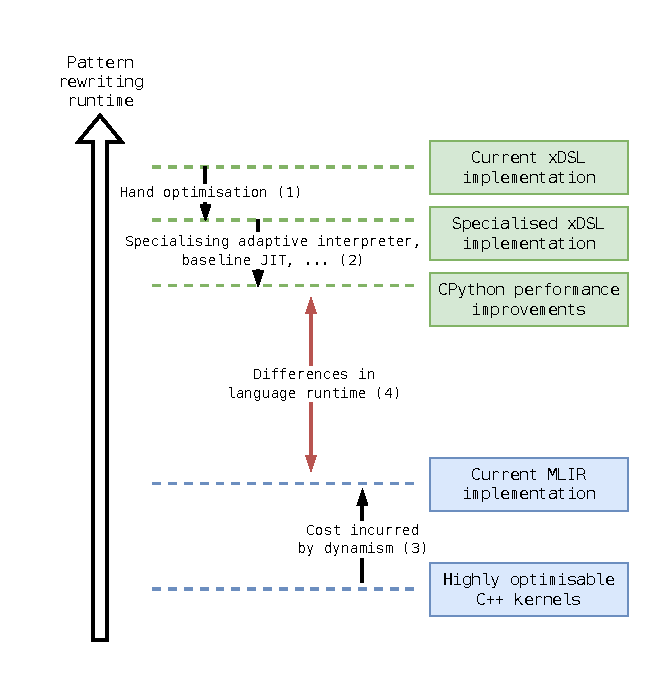
\includegraphics[width=0.75\textwidth]{images/11_introduction/narrative.drawio.pdf}
    \caption{Shrinking the gap between xDSL (green) and \ac{mlir} (blue) pattern rewriting performance. xDSL's performance can be improved by changes to its implementation and language runtime. MLIR has less of a performance advantage due to the costs associated with dynamism.} % TODO: Rework diagram presentation and substantiate. Perhaps this could be a bar chart, or at least annotated with real performance figures.
    \label{fig:narrative}
\end{figure}

% Hook (implementation details of Python)
% The performance of a program is upper bounded by properties of its language runtime, but is also significantly affected by the details of its implementation.
The performance of a program is constrained by both the details of its implementation and the runtime of its language.
% Argument
These two properties are deeply interlinked, making them difficult to independently measure. To mitigate this, we hand specialise (Label \texttt{(1)} of \autoref{fig:narrative}) xDSL's implementation for a specific workload such that its performance is constrained by the language runtime. The efficiency of this optimisation can then be examined through the dispatched bytecode for micro-benchmarks of this workload. Using this specialised implementation, we further quantify the impact of recent performance enhancements made to CPython including the specialising adaptive interpreter and baseline JIT (Label \texttt{(2)} of \autoref{fig:narrative}) for pattern rewriting workloads. In addition to this, the specialisation process and performance measurements provide insight into optimisations for the xDSL framework for general workloads.
% Link
The resultant specialised implementation leveraging recent CPython features can then be used as a baseline for best-case performance of pattern rewriting in xDSL in comparison with \ac{mlir}.


% Hook (cost of dynamism)
One of the key differences between xDSL's Python runtime and \ac{mlir}'s C++ runtime is their degree of dynamism.
% Argument
Being ahead-of-time statically compiled, C++ excels at workloads where control flow is known ahead of time, allowing optimisation and avoiding runtime overhead. However, the dynamism of pattern rewriting workloads forces frequent resolution of virtual function calls, hiding these optimisation opportunities and incurring overhead (Label \texttt{(3)} of \autoref{fig:narrative}).
CPython incurs this overhead of dynamism for almost all bytecode operations executed by its interpreter, irrespective of workload.
% Link
We examine the degree to which the dynamism in pattern rewriting workloads contributes to the differences in performance between language runtimes (Label \texttt{(4)} of \autoref{fig:narrative}), and critically assess the extent to which this motivates the use of Python for implementing user-extensible compiler frameworks.

% Hook (further optimisations)
% Argument
% Link

% \section{Contributions}
% \label{sec:contributions}
% % "give a brief overview of what you actually did"

The contributions of our work are as follows:

\begin{itemize}
    \item An examination of the upper bound on performance for pattern-rewriting workloads in the CPython language runtime, including trade-offs in expressivity and the impact of performance optimisations made to the language runtime.
    \item A tool to examine CPython bytecode dispatch in program runs, facilitating the analysis of costs incurred by dynamism 
    \item A quantitative comparison of the performance and impact of dynamism between user-extensible compiler frameworks implemented in static and dynamic languages.
    \item An exploration of optimisation techniques to shrink the performance gap between dynamic and static languages for pattern rewriting workloads.
\end{itemize}


% \textbf{xDSL benchmarks and benchmarking infrastructure.} We present a suite of benchmarks for the xDSL compiler framework. These examine end-to-end workloads, individual pipeline phases, and micro-benchmarks for frequent granular methods. These benchmarks are accompanied by infrastructure for their measurement and profiling. This includes supporting existing tooling such as air-speed velocity \cite{michaeldroettboomAirspeedvelocityAsv2025} for measuring performance regression, and hooks for profilers such as \texttt{viztracer} \cite{gaoVizTracer2025} and \texttt{cProfile}. In addition to this, we provide custom runtime measurement logic which minimises machine noise, and a novel tracing profiler which tracks the time taken to execute individual opcodes.

% \textbf{Comparison of xDSL and MLIR performance.} A subset of the above suite of benchmarks are designed to be directly comparable with existing micro-benchmarks for MLIR presented in the talk ``How Slow is MLIR?'' \cite{aminiHowSlowMLIR2024}. We present a comparison between the xDSL and MLIR frameworks using these micro-benchmarks. This comparison identifies two main causes for the disparity in performance between xDSL and MLIR: implementation overhead and language runtime overhead. By specialising the implementation of the micro-benchmarked methods to eliminate implementation overhead, we quantify the performance difference between the Python and C++ language runtimes for user-extensible compiler framework workloads.

% \textbf{Analysis of the suitability of dynamic languages for dynamic workloads.} User-extensible compiler frameworks are inherently dynamic, motivating the use of dynamic languages for their implementation. We identify examples of dynamism in our framework micro-benchmarks, and use them to evaluate whether dynamic language runtimes provide performance benefits for such dynamic workloads.
% TODO: We find that...

% \textbf{Optimisation of specialised xDSL pattern rewriter.}
% TODO: Still a slightly open question...
% Some benchmark informed changes are applicable wlog so can be/have been merged
% + possibly some bytecode rewriting stuff?